\section{Kiến thức nền tảng}
\subsection{Khảo sát thực tế}
\subsubsection{H\&M}

\indent \indent H\&M (Hennes \& Mauritz AB) là một tập đoàn thời trang quốc tế có trụ sở tại Thụy Điển. H\&M có mặt trên toàn thế giới và chuyên cung cấp các sản phẩm thời trang cho nam, nữ và trẻ em.

H\&M đã phát triển ứng dụng di động dành cho khách hàng có tên là "H\&M". Ứng dụng này cung cấp trải nghiệm mua sắm thuận tiện, cho phép người dùng duyệt qua các sản phẩm, thực hiện đặt hàng và nhận thông tin về khuyến mãi và xu hướng thời trang.
\subsubsection{Zalora}
\indent \indent Zalora là một công ty thương mại điện tử chuyên về thời trang có hoạt động rộng khắp khu vực Đông Nam Á.

Zalora cung cấp một ứng dụng di động cho phép khách hàng duyệt qua và mua sắm các sản phẩm thời trang từ các thương hiệu nổi tiếng.

Ứng dụng Zalora cung cấp các tính năng như tìm kiếm sản phẩm, xem chi tiết sản phẩm, đặt hàng và thanh toán trực tuyến.
\subsubsection{Cider}
\indent \indent Cider là một ứng dụng di động bán hàng thời trang phổ biến. Ứng dụng này cung cấp một nền tảng tương tác giữa người bán và người mua, cho phép người dùng tạo và quản lý cửa hàng trực tuyến của riêng mình.

Cider hỗ trợ việc tạo và quản lý danh mục sản phẩm, xử lý thanh toán, và tương tác với khách hàng thông qua hệ thống chat tích hợp.

\subsubsection{So sánh giữa các ứng dụng}
\begin{center}
\begin{longtable}{ |p{3cm}|p{3cm}|p{3cm}|p{3cm}| }
\hline
\textbf{Các tiêu chí}  & \textbf{H\&M \cite{HM}} & \textbf{ZALORA \cite{zalora}} & 
\textbf{CIDER \cite{cider}} \\
\hline
\endfirsthead

\hline
\textbf{Các tiêu chí}  & \textbf{H\&M \cite{HM}} & \textbf{ZALORA \cite{zalora}} & 
\textbf{CIDER \cite{cider}} \\
\hline
\endhead

\raggedright Giao diện người dùng (UI) và trải nghiệm người dùng (UX) &  Hiện đại và thân thiện với người dùng & Đẹp, dễ sử dụng, tốc độ phản hồi nhanh & Thiết kế đẹp, dễ sử dụng\\
\hline
\raggedright Tính năng sản phẩm & Đa dạng, xu hướng thời trang nhanh & Nhiều thương hiệu quốc tế và địa phương &Đa dạng, thời trang nhanh dành cho phụ nữ\\
\hline
\raggedright Tích hợp thanh toán và giao hàng & Thuận tiện & Có đầy đủ các tích hợp thanh toán & Có tích hợp thanh toán và giao hàng\\
\hline
\raggedright Tương tác xã hội và đánh giá & Không tích hợp xem đánh giá sản phẩm & Tích hợp đánh giá và phản hồi khách hàng & Tích hợp xem đánh giá sản phẩm, chia sẻ mạnh mẽ trên mạng xã hội\\
\hline
\raggedright Hiệu suất và tốc độ & Ứng dụng hoạt động mượt mà & Ứng dụng hoạt động mượt mà & Ứng dụng hoạt động mượt mà \\
\hline
\raggedright Tính năng tương tác & Danh sách mong muốn, lịch sử mua sắm, thông báo & Danh sách mong muốn, lịch sử mua sắm, thông báo & Có danh sách ưa thích. Không có thử đồ trực tuyến, tư vấn khác thời trang \\
\hline
\raggedright Hỗ trợ khách hàng & Trung tâm trợ giúp, chat trực tiếp, email & Có hỗ trợ khách hàng trực tuyến & Không có hỗ trợ khách hàng\\
\hline
\raggedright Tìm kiếm thông minh & Theo tên, danh mục, bộ sưu tập & Dựa theo từ khóa tìm kiếm nhiều nhất & Dựa theo từ khóa\\
\hline
\raggedright Hệ thống gợi ý mua hàng & Dựa trên lịch sử mua sắm & Dựa trên lịch sử mua sắm & Dựa trên lịch sử mua sắm \\
\hline
\caption{Bảng so sánh các tiêu chí}
\end{longtable}
\end{center}
Mô tả các tiêu chí:
\begin{itemize}
    \item Giao diện người dùng (UI) và trải nghiệm người dùng (UX): Đánh giá cách ứng dụng được thiết kế và cách người dùng tương tác với nó. Giao diện nên dễ sử dụng, hấp dẫn và phản ánh thương hiệu.

 \item Tính năng sản phẩm: Đảm bảo rằng ứng dụng cung cấp đầy đủ thông tin về sản phẩm, bao gồm hình ảnh, mô tả chi tiết và giá cả. Các tính năng như tìm kiếm, lọc sản phẩm và đánh giá sản phẩm cũng nên được cung cấp.

\item Tích hợp thanh toán và giao hàng: Kiểm tra tính năng thanh toán an toàn và đa dạng cùng với tùy chọn giao hàng linh hoạt. Bảo đảm rằng thông tin thanh toán của khách hàng được bảo vệ.

\item Tương tác xã hội và đánh giá: Ứng dụng nên cho phép khách hàng đăng nhận xét và đánh giá sản phẩm. Cung cấp tích hợp xã hội để chia sẻ sản phẩm và khuyến mãi.

\item Tính năng tương tác: Cân nhắc tích hợp tính năng thử đồ trực tuyến, hoặc tạo các chức năng tương tác khác như tư vấn thời trang hoặc danh sách ưa thích.

\item Tính năng phân tích và theo dõi: Đánh giá khả năng theo dõi hoạt động của người dùng, thống kê doanh số bán hàng, và sử dụng các công cụ phân tích để cải thiện chiến lược kinh doanh.

\item Bảo mật và quyền riêng tư: Đảm bảo rằng thông tin cá nhân của khách hàng được bảo vệ một cách an toàn và tuân thủ các quy định về quyền riêng tư.

\item Hiệu suất và tốc độ: Ứng dụng nên hoạt động một cách nhanh chóng và mượt mà trên các thiết bị khác nhau.

\item Hỗ trợ khách hàng: Cung cấp các kênh hỗ trợ khách hàng như chat trực tuyến, email hoặc số điện thoại để giải quyết thắc mắc và vấn đề của khách hàng.

\item Tích hợp mạng xã hội và tiếp thị: Đánh giá khả năng chia sẻ trên mạng xã hội và các chiến dịch tiếp thị trên ứng dụng.

\item Tuân thủ quy định: Đảm bảo rằng ứng dụng tuân thủ tất cả các quy định và luật pháp liên quan đến kinh doanh trực tuyến và bán hàng.
\end{itemize}

% \subsection{Các khái niệm trong hệ thống}

\subsection{Cơ sở lý thuyết}
\subsubsection{Kiến trúc phân lớp (Layered Architecture)}
\indent \indent Kiến trúc phân lớp là một phương pháp tổ chức và xây dựng hệ thống phần mềm, trong đó các thành phần được chia thành các lớp riêng biệt với vai trò và trách nhiệm cụ thể. Mỗi lớp đảm nhận một phần công việc cụ thể và tương tác với các lớp khác thông qua giao diện định nghĩa rõ ràng.

\begin{figure}[H]
    \centering
    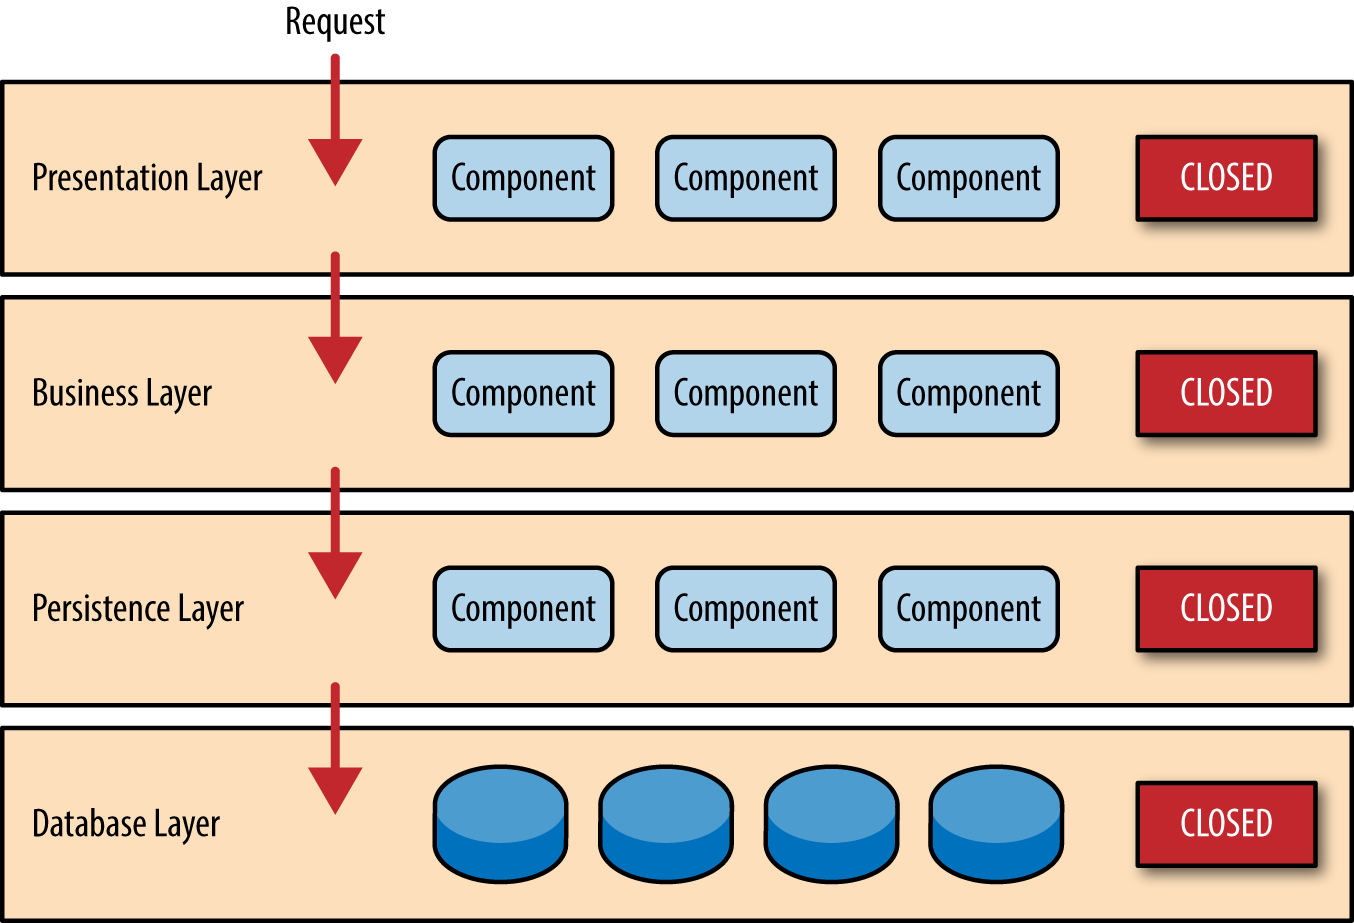
\includegraphics[width=15cm]{Images/Technology/layer_ar.png}
    \vspace{1cm}
    \caption{Four Layered Architecture \cite{layerd}}
\end{figure}

\noindent Trong kiến trúc phân lớp, hệ thống được chia thành ba lớp chính:
\begin{itemize}
    \item \textbf{Presentation layer} (lớp giao diện): Đây là lớp mà người dùng tương tác trực tiếp. Nó xử lý việc hiển thị dữ liệu và tương tác với người dùng thông qua giao diện người dùng.
    \item \textbf{Business layer} (lớp logic): Lớp này chứa các quy tắc nghiệp vụ và xử lý logic của hệ thống. Nó đảm bảo tính logic và tính toàn vẹn của dữ liệu.
    \item \textbf{Data layer} (lớp dữ liệu): Lớp này quản lý truy cập và tương tác với cơ sở dữ liệu. Nó cung cấp các phương thức để lấy và lưu trữ dữ liệu.
\end{itemize}
Trong dự án này chúng tôi sẽ dùng thêm một lớp là 
\textbf{Persistence Layer}, thường là một phần của Business Layer. Nó cung cấp các dịch vụ để tương tác với cơ sở dữ liệu, bao gồm các hoạt động như truy vấn, cập nhật, xóa và tạo mới dữ liệu. Qua tầng này, các thành phần trong Business Layer có thể giao tiếp với cơ sở dữ liệu một cách đơn giản và trừu tượng hóa. Với việc gọi Persistence Layer, chúng ta có thể truy xuất và sửa đổi dữ liệu trong cơ sở dữ liệu một cách dễ dàng và linh hoạt. Chúng tôi có sử dụng các công nghệ như ORM (Object-Relational Mapping) và OGM (Object-Graph Mapping) để tạo ra các đối tượng và ánh xạ chúng thành dữ liệu trong cơ sở dữ liệu. Điều này giúp tách biệt logic kinh doanh và tương tác với cơ sở dữ liệu, tạo ra một kiến trúc dễ bảo trì và mở rộng.
Các lớp trong kiến trúc phân lớp được tổ chức theo cách mà mỗi lớp chỉ phụ thuộc vào lớp ngay dưới nó, và không phụ thuộc vào lớp ngay trên nó. Điều này giúp tách biệt các công việc và trách nhiệm của từng lớp và dễ dàng thay đổi và bảo trì hệ thống.

Kiến trúc phân lớp giúp tăng tính linh hoạt, tái sử dụng và bảo trì của hệ thống phần mềm. Nó cũng giúp tách biệt các quy tắc nghiệp vụ và giao diện người dùng, làm cho hệ thống dễ dàng mở rộng và thay đổi theo yêu cầu của người dùng.
\subsubsection{RESTful API}
RESTful API (Representational State Transfer - Application Programming Interface) là một kiến trúc thiết kế API dựa trên các nguyên tắc của REST, giúp tạo ra các dịch vụ web mạnh mẽ, linh hoạt và dễ hiểu. RESTful API thường được sử dụng để tương tác với cơ sở dữ liệu và tạo ra các ứng dụng web hoặc di động.\\
Đặc Điểm và Tính Năng Chính của RESTful API:
\begin{itemize}
\item HTTP Methods: RESTful API sử dụng các phương thức HTTP như GET, POST, PUT, PATCH, và DELETE để thực hiện các thao tác trên tài nguyên. Mỗi phương thức có ý nghĩa và mục đích riêng.
\item Stateless Communication: Giao tiếp trong RESTful API là stateless, điều này có nghĩa là mỗi yêu cầu từ client đều chứa đủ thông tin cần thiết để server hiểu và xử lý mà không cần dựa vào bất kỳ trạng thái nào từ trước đó.
\item Resource-Based: Mọi thứ trong RESTful API được xem như một tài nguyên và được định danh bằng các URI (Uniform Resource Identifier). Điều này giúp dễ dàng quản lý và tìm kiếm các tài nguyên.
\item Representation: Dữ liệu của tài nguyên được truyền tải giữa client và server dưới dạng các biểu diễn (representation) như JSON hoặc XML. Điều này giúp tương thích và linh hoạt.
\item HATEOAS (Hypermedia As The Engine Of Application State): RESTful API có thể cung cấp các liên kết hypermedia trong các phản hồi, giúp client hiểu được các hành động mà nó có thể thực hiện tiếp theo.
\item Versioning: RESTful API thường hỗ trợ việc quản lý phiên bản để đảm bảo tính tương thích giữa các phiên bản khác nhau của API.
\item Authentication và Authorization: RESTful API hỗ trợ các phương thức xác thực và phân quyền để đảm bảo an toàn và bảo mật thông tin.
\item Caching: RESTful API có thể sử dụng các cơ chế caching để tối ưu hóa hiệu suất, giảm tải cho server, và giảm thời gian đáp ứng\\
RESTful API đã trở thành một tiêu chuẩn phổ biến trong việc xây dựng các dịch vụ web và ứng dụng di động, đặc biệt là khi cần sự tương thích và khả năng mở rộng.
\end{itemize}
\subsubsection{Json Web Token}
\begin{figure}[h]
    \centering
    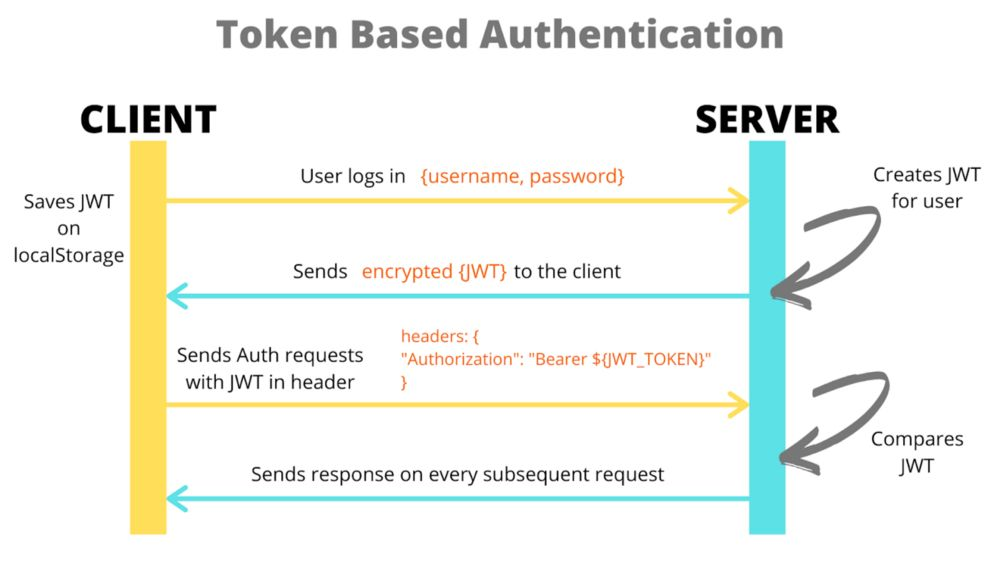
\includegraphics[width=10cm]{Images/Technology/jwt.png}
    \vspace{10pt}
    \caption{Json Web Token \cite{jsonwebtoken}}
\end{figure}

JSON Web Token (JWT) là một tiêu chuẩn mở định nghĩa một cách ngắn gọn và khép kín
để truyền dẫn thông tin giữa hai bên client và server được định dạng bằng JSON.\\
Chuỗi JWT gồm 3 thành phần là header, payload, signature và được ngăn cách nhau bằng
dấu chấm ("."). Do đó, một chuỗi JWT có dạng như sau:
\begin{center}
    \textbf{header.payload.signature}
\end{center}
\begin{itemize}
    \item \textbf{Header}: Phần header thường chứa hai phần là kiểu dữ liệu (giá trị thường là JWT) và thuật toán sử dụng để mã hóa chuỗi như HMAC SHA256 hoặc RSA.
    \item \textbf{Payload}:Phần payload chứa thông tin muốn đặt trong chuỗi như tên đăng nhập (username), id của người dùng (user id), tên người dùng,...
    \item \textbf{Signature}: Phần signature sẽ được tạo ra bằng cách mã hóa phần header và payload kèm theo một chuỗi được gọi là secret (khóa bí mật). Thuật toán để mã hóa được mô tả ở phần header.
    
\end{itemize}
\subsubsection{Graph}
\
\indentĐồ thị là một tập các đối tượng gọi là đỉnh nối với nhau bởi các cạnh. Thông thường, đồ thị được vẽ dưới dạng một tập các điểm (đỉnh, nút) nối với nhau bởi các đoạn thẳng (cạnh). Graph Database mô tả và lưu trữ dữ liệu dưới dạng đồ thị, một cách trực quan và dễ dàng truy vấn. Hiểu 1 cách đơn giản, graph database là database sử dụng cấu trúc graph để lưu trữ dữ liệu, nó khác so với cơ sỡ dữ liệu quan hệ lưu data dưới dạng bảng, hay NoSQL lưu data dưới dạng document key value.
\begin{figure}[h]
    \centering
    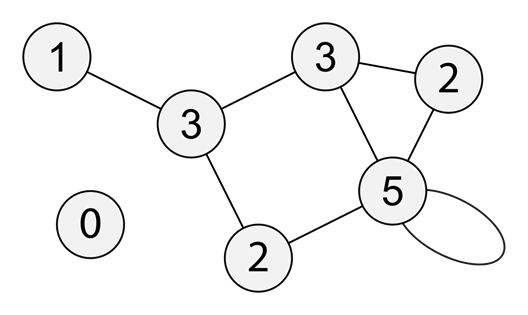
\includegraphics[width=7cm]{Images//Technology/graph.png}
    \vspace{10pt}
    \caption{Graph \cite{graph}}
    \label{fig:enter-label}
\end{figure}
\\
\noindent\textbf{Lợi ích của Graph}\\
\indent Bối cảnh hiện đại đặt ra rất nhiều bài toán cần phải giải quyết như: phát hiện gian lận tài chính, gợi ý bạn bè trên các nền tảng mạng xã hội, gợi ý một item cho người dùng dựa trên lịch sử hoạt động của người đó...\\
\indent Với những kiểu bài toán như vậy thì cách lưu trữ dữ liệu của Relational Database hoặc NoSQL Database đều không thích hợp khi mà chúng chỉ chuẩn hóa dữ liệu để lưu vào các bảng hay các document và làm giảm đi tính kết nối. Việc lưu trữ như vậy không thể tận dụng được hết sức mạnh của các mối liên kết có thể mang lại. Đặc biệt, việc truy vấn giữa các bảng rất phức tạp và mất nhiều thời gian.\\
Một minh chứng cho sự hữu ích của Graph Database đó chính là việc gợi ý kết bạn trên nền tảng mạng xã hội Facebook. Ví dụ, khi A là bạn của B và B là bạn của C, với công nghệ graph, Facebook sẽ biết được liệu có nên gợi ý kết bạn cho A và C hay không.\\
\noindent \textbf{Một số bài toán áp dụng Graph Database}
\begin{itemize}
    \item Xây dựng một hệ thống gợi ý mua hàng thông qua các mối quan hệ giữa người dùng A và B khi có điểm tương đồng trong việc mua sản phẩm.
    \item Phát hiện mối liên hệ giữa những người dùng có quen biết nhau, có tương tác giống nhau trên mạng xã hội.
    \item Phát hiện các hành vi vi phạm tài chính, ví dụ như hành vi rửa tiền khi chuyển khoản qua nhiều tài khoản, nhiều ngân hàng khác nhau.
    \item Gợi ý kết bạn dựa trên mối quan hệ bạn bè hiện có của tài khoản mạng xã hội
    \item Tối ưu đường bay của máy bay thương mại, tối ưu đường vận tải của các xe chở hàng

\end{itemize}
\subsection{Công nghệ}
\subsubsection{Công nghệ Frontend}
\begin{enumerate}[a. ]
\item \textbf{Typescript}\\
\begin{figure}[H]
    \centering
     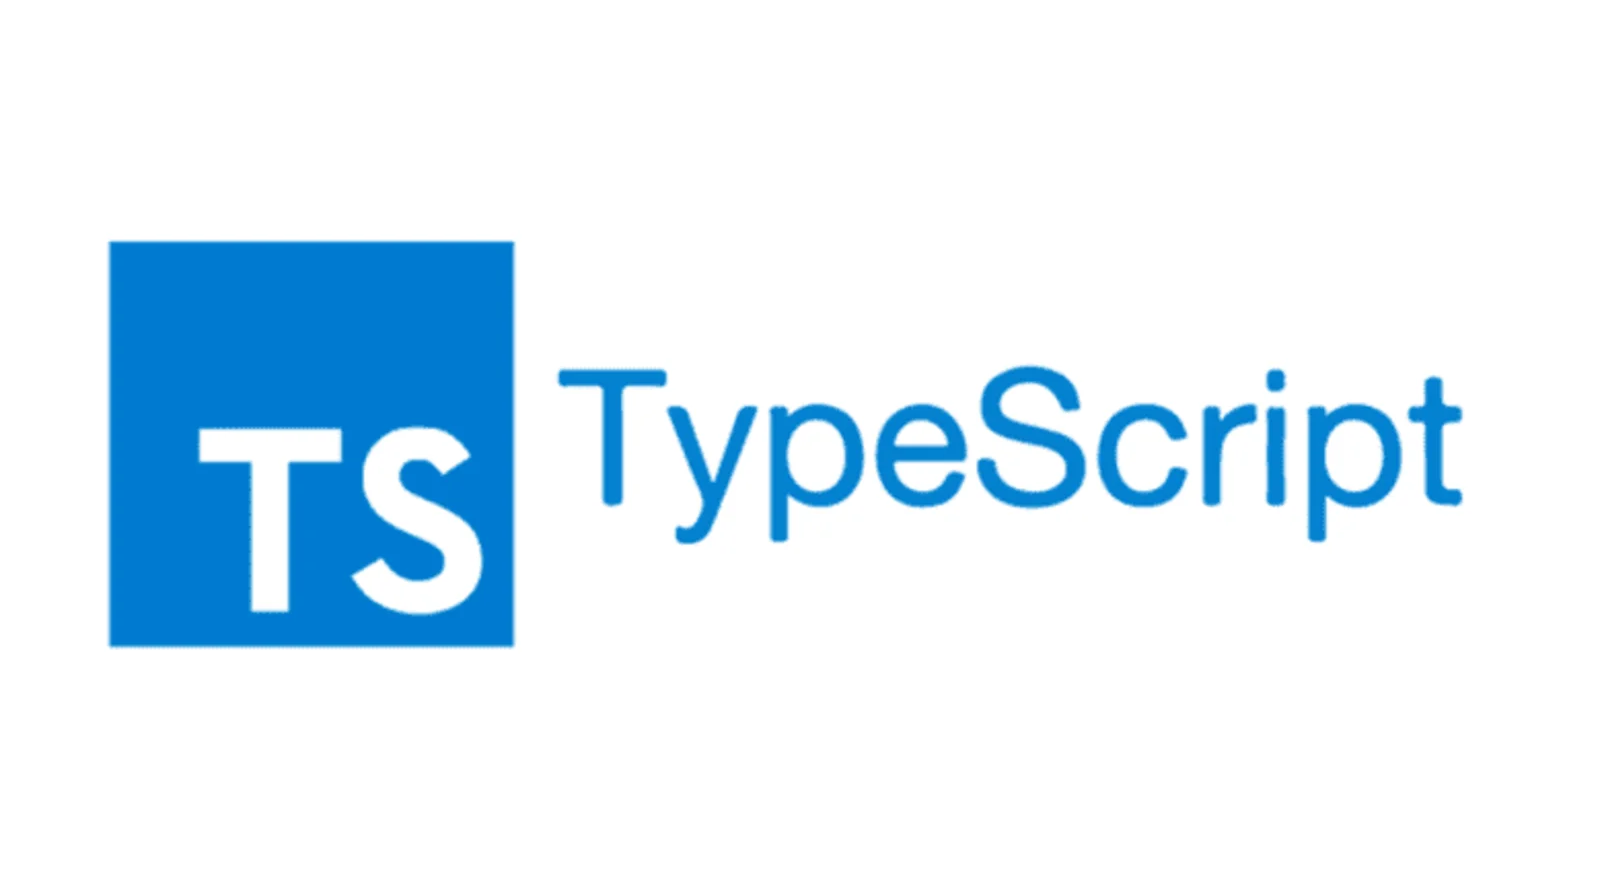
\includegraphics[scale=0.15]{Images/Technology/ts1.png}
     \caption{TypeScript \cite{typescript}}
\end{figure}
TypeScript là một ngôn ngữ lập trình mã nguồn mở được phát triển bởi Microsoft, và nó có thể được coi là một "mở rộng" của JavaScript. TypeScript được tạo ra để giúp việc phát triển ứng dụng JavaScript lớn và phức tạp trở nên dễ dàng hơn bằng cách thêm vào nó các khái niệm về kiểu dữ liệu tĩnh và các tính năng lập trình hướng đối tượng. \\
Đặc điểm và tính năng chính của TypeScript:
\begin{itemize}
\item Kiểu dữ liệu tĩnh: TypeScript giúp xác định rõ kiểu dữ liệu của biến, tham số hàm và giá trị trả về của hàm. Điều này giúp phát hiện lỗi kiểu tại thời điểm biên dịch thay vì tại thời điểm chạy, giúp tăng tính ổn định và tin cậy của ứng dụng.
\item Lập trình hướng đối tượng: TypeScript hỗ trợ các khái niệm lập trình hướng đối tượng như lớp, đối tượng, kế thừa, và các tính năng khác. Điều này giúp tạo ra mã nguồn dễ hiểu, tái sử dụng và bảo trì.
\item Tích hợp với JavaScript: TypeScript là siêu tập của JavaScript, nghĩa là mọi mã JavaScript hợp lệ đều là mã TypeScript. Điều này cho phép dự án chuyển từ JavaScript sang TypeScript một cách dễ dàng và mục tiêu đặt ra là giữ nguyên tương thích ngược.
\item Compiler: TypeScript có một trình biên dịch riêng biệt, giúp kiểm tra và chuyển đổi mã nguồn TypeScript thành mã nguồn JavaScript. Quá trình biên dịch này giúp kiểm soát lỗi và tối ưu hóa mã nguồn.
\end{itemize}

\item \textbf{ReactJs}\\
\begin{figure}[H]
    \centering
     
\includegraphics[scale=0.15]{Images/Technology/react.png}
     \vspace{10pt}
     \caption{React \cite{reactjs}}
\end{figure}
React JS là một thư viện JavaScript phổ biến do Facebook phát triển, dùng để xây dựng giao diện người dùng (UI).\\
Tính năng chính của React JS:
\begin{itemize}
\item Component-Based: React cho phép tạo các đơn vị UI tái sử dụng gọi là "Components," mỗi cái có logic và cấu trúc riêng, có thể tái sử dụng ở nhiều nơi khác nhau trong ứng dụng.
\item Hiệu suất: Sử dụng Virtual DOM để cập nhật và đồng bộ hóa trạng thái DOM hiệu quả, giúp cập nhật UI nhanh chóng và mượt mà.
\item JSX: React sử dụng cú pháp mở rộng của JavaScript, JSX, cho phép tích hợp logic và render markup trong cùng một component.
\item Kết hợp dễ dàng: React hoạt động tốt với các thư viện và framework khác, có thể sử dụng làm view layer trong các ứng dụng MVC.
\end{itemize}
\item \textbf{React Native}
\begin{figure}[H]
    \centering
     
\includegraphics[scale=0.3]{Images/Technology/reactNative.png}
     \vspace{10pt}
     \caption{React Native \cite{reactnative}}
     \label{fig:enter-label}
\end{figure}
React Native là một framework mã nguồn mở được phát triển bởi Facebook. Framework này giúp phát triển app mobile trên cả 2 hệ sinh thái iOS và Android một cách dễ dàng. Chính vì thế lập trình React Native sẽ giúp tiết kiệm được phần lớn thời gian và công sức khi thiết kế và xây dựng nên một ứng dụng đa nền tảng.\\\\
\textbf{Những ưu điểm của React Native}
\begin{itemize}
\item  Thời gian học React Native ngắn: 
React Native cung cấp giải pháp lập trình đa nền tảng. Thay vì tìm hiểu 2 hệ sinh thái các biệt của iOS và Android, chỉ tốn thời gian học React Native có thể phát triển tốt cho cả iOS và Android.
\item Có thể lập trình trên đa dạng hệ điều hành:
React Native là bước chuyển mình lớn của mobile app. Việc lập trình trên đa dạng hệ điều hành mang đến sự tiện ích cho cộng đồng dev trên toàn cầu.
\item Cộng đồng React Native lớn:
React Native được rất nhiều ông lớn trong ngành công nghệ đang sử dụng. Điều này giúp cho cộng đồng người học React Native phát triển mạnh mẽ.
\item Hot Reloading:
Với mỗi lập trình viên, thời gian Reload app sau mỗi chỉnh sửa nhỏ luôn là vấn đề khó chịu và tốn nhiều thời gian. Trong nhiều project với lượng source code lớn thì thời gian build, đóng gói và cài đặt lại luôn gây mệt mỏi đối với dev. Đặc biệt là trong giai đoạn dự án gấp rút.
\item Tăng trải nghiệm của người dùng:
Giao diện đơn giản, đa dạng ứng dụng, hoàn hảo trong thiết kế app… React Native tạo nên nhiều ứng dụng hữu ích cho người dùng. Hàng nghìn ứng dụng đang dùng React Native chính là minh chứng cho sự linh hoạt của ứng dụng từ React Native.
\end{itemize}
% \item \textbf{Flutter}
% \begin{figure}[H]
% \centering
%  
\includegraphics[scale=0.35]{Images/Technology/flutter.png}
% \end{figure}
% Flutter là một framework phát triển ứng dụng di động mã nguồn mở được phát triển bởi Google. Được giới thiệu vào năm 2017, Flutter nhanh chóng trở thành một lựa chọn phổ biến cho việc xây dựng ứng dụng di động đa nền tảng, với khả năng chia sẻ mã nguồn giữa các nền tảng khác nhau.\\
% Flutter sử dụng ngôn ngữ lập trình Dart và nổi bật với mô hình lập trình gọi là "reactive programming," trong đó giao diện người dùng được xây dựng dựa trên trạng thái và sự kiện. Framework này cung cấp một tập hợp đầy đủ các widget để xây dựng giao diện người dùng, giúp ứng dụng có giao diện thân thiện và đẹp mắt.\\
% Flutter cho phép phát triển ứng dụng không chỉ cho nền tảng di động (iOS và Android) mà còn cho web và desktop. Điều này mang lại sự linh hoạt và tiện ích trong việc đáp ứng nhu cầu ngày càng đa dạng của người phát triển.\\
% Đặc Điểm và Tính Năng Chính của Flutter:
% \begin{itemize}
% \item Widget-Based: Flutter sử dụng mô hình lập trình dựa trên widget, cho phép xây dựng giao diện người dùng từ các thành phần nhỏ gọi là widget. Điều này giúp tái sử dụng mã nguồn và xây dựng giao diện phức tạp.
% \item Hot Reload: Flutter hỗ trợ tính năng Hot Reload, cho phép nhà phát triển thấy ngay lập tức các thay đổi trong ứng dụng mà không cần khởi động lại. Điều này giúp nhanh chóng thử nghiệm và phát triển ứng dụng.
% \item Dart Programming Language: Flutter sử dụng ngôn ngữ lập trình Dart, được tối ưu hóa cho việc xây dựng ứng dụng di động. Dart kết hợp tính năng của các ngôn ngữ khác như Java và JavaScript.
% \item Giao Diện Đẹp Mắt và Linh Hoạt: Flutter cung cấp một loạt các widget giúp tạo ra giao diện người dùng đẹp mắt và linh hoạt. Sự tương thích cao giữa các thiết bị và nền tảng khác nhau giúp đảm bảo trải nghiệm người dùng nhất quán.
% \item Phát triển Đa Nền Tảng: Flutter cho phép phát triển ứng dụng cho nhiều nền tảng, bao gồm iOS, Android, web và desktop, giúp giảm chi phí phát triển và duy trì.
% \item Cộng Đồng và Hỗ Trợ Đa Dạng: Flutter có một cộng đồng đông đảo và tích cực, cung cấp nhiều tài nguyên, thư viện và công cụ hỗ trợ để giúp nhà phát triển xây dựng ứng dụng hiệu quả và mạnh mẽ
% \end{itemize}
% \newpage
\item \textbf{Material UI}
\begin{center}
    \begin{figure}[H]
            \centering
             
\includegraphics[scale=0.15]{Images/Technology/MUI.png}            
             \caption{Material UI \cite{mui}}
             \label{fig:enter-label}
        \end{figure}
\end{center}
Material-UI là một thư viện giao diện người dùng (UI) phát triển dựa trên nguyên tắc của "Material Design" của Google. Được xây dựng cho React, Material-UI cung cấp một bộ công cụ mạnh mẽ cho việc xây dựng giao diện người dùng hiện đại và hấp dẫn.\\
Đặc điểm và tính năng chính của Material-UI:
\begin{itemize}
\item Bộ các component đa dạng: Material-UI cung cấp một loạt các component như buttons, input fields, navigation bars, và nhiều hơn nữa. Các component này được xây dựng để có tính tương thích và linh hoạt cao.
\item Tùy biến dễ dàng: Mỗi component trong Material-UI có thể được tùy biến dễ dàng thông qua các prop và CSS-in-JS styling, giúp phát triển tạo ra giao diện người dùng theo ý muốn.
\item Hỗ trợ Theme và Styles: Material-UI hỗ trợ quản lý theme, cho phép tùy chỉnh toàn bộ giao diện người dùng của ứng dụng một cách dễ dàng. Nó cũng tích hợp các hệ thống quản lý styles để giúp tạo ra mã nguồn gọn gàng và dễ đọc.
\item Tương thích React: Material-UI là một thư viện React, giúp tích hợp dễ dàng vào dự án React hiện tại và sử dụng cùng với các tính năng của React như props, state, và lifecycle methods.

\end{itemize}


\end{enumerate}
\subsubsection{Công nghệ Backend}
\begin{enumerate}[a.]
\item \textbf{NodeJS}\\
Là một môi trường (JavaScript Runtime Environment), đa nền tảng,
mã nguồn mở, dùng để thực thi mã JavaScript bên ngoài trình duyệt web. Node.js được thiết kế để xây dựng các ứng dụng mạng có tính mở rộng cao. Node.js sử dụng engine JavaScript V8 của Google để thực thi mã và được xây dựng dựa trên thư viện libuv.
\\
\begin{figure}[H]
    \centering
    
\includegraphics[width=10cm]{Images//Technology/Nodejs.png}
    \vspace{10pt}
    \caption{NodeJS \cite{nodejs}}
    \label{fig:enter-label}
\end{figure}
Một số tính năng chính của Node.js:
\begin{itemize}
    \item  Hiệu suất: Node.js rất hiệu quả trong việc xử lý các yêu cầu đồng thời (song song). Điều này là do Node.js sử dụng Event Loop đơn luồng để xử lý tất cả các yêu cầu. Điều này có nghĩa là Node.js có thể xử lý một số lượng lớn yêu cầu cùng lúc mà không bị tranh chấp tài nguyên.
    \item Cộng đồng: Node.js có một cộng đồng các nhà phát triển lớn và tích cực. Điều này có nghĩa là có nhiều tài nguyên dành cho nhà phát triển Node.js, chẳng hạn như hướng dẫn, tài liệu và packages.
    \item  Có khả năng tương thích với các công nghệ khác: Node.js có khả năng tương thích với các công nghệ khác như React, Angular và Vue, giúp cho việc phát triển ứng dụng trở nên dễ dàng hơn.
    \item  Có thể tích hợp với các cơ sở dữ liệu khác nhau: Node.js hỗ trợ tích hợp với các cơ sở dữ liệu khác nhau như MySQL, MongoDB, PostgreSQL, Redis, và nhiều loại cơ sở dữ liệu khác.
    \item Có hệ sinh thái Framework phong phú: Node.js có một hệ sinh thái phát triển rộng lớn với nhiều framework và thư viện phát triển ứng dụng như Express, Hapi, Koa, Meteor, NestJS, Loopback, và nhiều loại framework khác.
\end{itemize}

\item \textbf{ExpressJS}\\
Là một framework phát triển ứng dụng web dựa trên Node.js. Nó được thiết kế để đơn giản hóa việc xây dựng các ứng dụng web, cho phép các nhà phát triển tập trung vào việc phát triển các tính năng và chức năng của ứng dụng thay vì phải quan tâm đến các vấn đề cơ bản như routing và middleware.\\
\begin{figure}[H]
    \centering
    
\includegraphics[width=7cm]{Images//Technology/expressJs.png}
    \vspace{20pt}
    \caption{ExpressJS \cite{express}}
\end{figure}
Một số tính năng chính của Express.js:
\begin{itemize}
    \item  Routing: Express.js cung cấp một cách tiếp cận đơn giản và trực quan để xử lý các yêu cầu HTTP, các tác vụ CRUD (Create - Retrieve - Update - Delete), và định tuyến chúng đến các hàm xử lý tương ứng.
    \item Middleware: Middleware là một tính năng rất quan trọng của Express.js. Nó cho phép chèn các chức năng xử lý trung gian vào quá trình xử lý yêu cầu. Điều này cho phép thêm các tính năng như xác thực, kiểm tra lỗi, ghi log, tích hợp cả middleware của các ứng dụng/thư viện bên thứ ba và nhiều hơn nữa vào quá trình xử lý yêu cầu một cách dễ dàng.
    \item  Phù hợp với RESTful API: Là một trong những lựa chọn hàng đầu cho việc xây dựng RESTful API, nhờ tính linh hoạt của nó trong việc xử lý các yêu cầu HTTP và định tuyến chúng đến các hàm xử lý tương ứng.

\end{itemize}

\item \textbf{Prisma}\\
Prisma là một công cụ ORM (Object-Relational Mapping) hiệu quả được phát triển để làm cho việc làm việc với cơ sở dữ liệu trở nên dễ dàng và linh hoạt hơn. Được xây dựng dựa trên TypeScript và JavaScript, Prisma cung cấp một cách hiện đại để tương tác với cơ sở dữ liệu từ các ứng dụng Node.js.\\
\begin{figure}[H]
    \centering
    
\includegraphics[width=0.5\linewidth]{Images//Technology/prisma.png}
    \vspace{10pt}
    \caption{Prisma \cite{prisma}}
\end{figure}

Đặc điểm và tính năng chính của Prisma:
\begin{itemize}
\item Type-Safe Query Builder: Prisma sử dụng một Query Builder type-safe, cho phép tạo câu truy vấn cơ sở dữ liệu bằng cách sử dụng mã TypeScript. Điều này giúp giảm thiểu lỗi tại thời điểm chạy và tăng tính dễ bảo trì.
\item Auto-Generated Database Client: Prisma tạo ra một client cơ sở dữ liệu tự động từ schema, giúp đơn giản hóa sự tương tác với cơ sở dữ liệu. Việc này giúp tránh tình trạng khai báo các phương thức truy vấn thủ công.
\item Schema Migrations: Prisma hỗ trợ việc quản lý và triển khai các phiên bản schema của cơ sở dữ liệu một cách dễ dàng thông qua migrations. Điều này giúp duy trì phiên bản cơ sở dữ liệu theo cách an toàn và hiệu quả.
\item Đa cơ sở dữ liệu: Prisma không chỉ hỗ trợ một loạt các cơ sở dữ liệu quan hệ (như MySQL và PostgreSQL), mà còn có kế hoạch hỗ trợ cơ sở dữ liệu không quan hệ như MongoDB.

\end{itemize}
\item \textbf{PosgreSQL}\\
PostgreSQL (tên viết tắt từ "Postgres") là một hệ quản trị cơ sở dữ liệu (DBMS) mã nguồn mở và có tính năng đầy đủ. Nó được thiết kế để hỗ trợ một loạt các ứng dụng từ nhỏ đến lớn, từ dự án cá nhân đến các hệ thống doanh nghiệp quy mô lớn. PostgreSQL cung cấp một số tính năng mạnh mẽ và tiên tiến trong lĩnh vực quản lý cơ sở dữ liệu, và nó thường được sử dụng làm một lựa chọn cho các dự án đòi hỏi tính mở rộng và hiệu suất cao.
\begin{figure}[H]
    \centering
    
\includegraphics[width=10cm]{Images/Technology/posgres.png}
    \caption{PostgreSQL \cite{postgresql}}
\end{figure}
Đặc điểm và tính năng chính của MySQL:
\begin{itemize}
\item Tính an toàn và bảo mật: PostgreSQL có các tính năng mạnh mẽ về an toàn và bảo mật, bao gồm quản lý người dùng và phân quyền, các biện pháp bảo mật về mức cơ sở dữ liệu và giao tiếp, và khả năng kiểm soát truy cập.
\item Hiệu suất: PostgreSQL được thiết kế để cung cấp hiệu suất cao và có thể được tối ưu hóa cho nhiều tình huống sử dụng khác nhau.
\item Hỗ trợ mở rộng: PostgreSQL hỗ trợ nhiều tính năng mở rộng như replication (nhân bản dữ liệu), partitioning (phân vùng dữ liệu), và có thể tích hợp với các công nghệ mở rộng như PostgreSQL Foreign Data Wrappers (FDW) để truy cập dữ liệu từ các nguồn khác.
\end{itemize}    
\item \textbf{Neo4J}\\
\indent Neo4j là hệ quản trị cơ sở dữ liệu đồ thị, được giới thiệu đầu tiên vào năm 2007 và công bố phiên bản 1.0 vào năm 2010. Hiện nay, neo4j là một trong các cơ sở dữ liệu đồ thị mã nguồn mở phổ biến nhất. Neo4j hỗ trợ ngôn ngữ truy vấn Cypher, một ngôn ngữ rất trực quan trong việc truy vấn dữ liệu dưới dạng Graph.\\
\noindent \textbf{Ưu điểm của Neo4j}
\begin{itemize}
    \item Biểu diễn kết nối rất dễ dàng
    \item Việc truy xuất / duyệt / điều hướng nhiều dữ liệu dễ dàng và nhanh chóng hơn.
    \item Mô tả dữ liệu bán cấu trúc rất dễ dàng.
    \item Các lệnh ngôn ngữ truy vấn Neo4j ở định dạng dễ đọc và rất dễ học.
    \item Sử dụng mô hình dữ liệu đơn giản và mạnh mẽ.
    \item Khong yêu cầu các Joins phức tạp để truy xuất dữ liệu được kết nối / liên quan vì rất dễ dàng truy xuất các chi tiết mối quan hệ hoặc nút liền kề của nó mà không có Joins hoặc Indexes.
\end{itemize}
\end{enumerate}
